\chapter{Stiffness evolution of granular layers \\and the origin of repetitive, slow, \\stick-slip frictional sliding}

\section{Abstract}
We demonstrate the frictional behaviors of steady state sliding, stick-slip, and
repetitive, slow stick-slip sliding through a carefully-designed suite of
laboratory experiments focused on exploring the role of loading system stiffness
in controlling the frictional response to shear. We performed tests on sheared
layers of baking flour, with three configurations of loading blocks made of
steel and cast acrylic to achieve different stiffnesses. Slide-hold-slide and
velocity step tests were conducted and analyzed in a rate-and-state friction
framework. With compliant loading blocks, the material exhibits unstable
stick-slip behavior with slow-slip events of duration up to twenty seconds.
Slow-slip has been difficult to achieve in the lab and has only been observed
for a narrow variety of boundary conditions and materials. Our results suggest
that this behavior is strongly controlled by the stiffness of the system, the
strain history of the sample, and shear fabric evolution. We describe a new
suite of automated tools that greatly improve friction analysis and provide
insight to the underlying mechanisms of slow stick-slip. We demonstrate that
layer stiffness evolves with shear strain and modifies the mechanical behavior
of stick-slip sliding. Our work suggests that slow earthquakes in tectonic fault
zones may be linked to shear fabric development and associated changes in local
stiffness, likely in combination with variations in frictional constitutive
properties and effective stress.

\section{Introduction}
Although stick-slip is generally considered an analog for earthquakes
\cite{Brace_Byerlee_1969,Johnson_2013} in the framework of stable or unstable
sliding, it has recently become evident that there is a spectrum of fault slip
behaviors \cite{peng2010integrated}.  The discovery of slow earthquakes and
non-volcanic tremor \cite{ikari2013slip,Beroza:2011jk,obara2002nonvolcanic,ide2007mechanism}
has raised questions about the link between fault zone frictional properties, in
situ conditions, and the underlying mechanisms of slow-slip
\cite{kaproth2013slow}.

The rate and state frictional model provides a convenient framework in which to
examine the frictional response of materials and characterize their second order
frictional characteristics that are thought to control the stability of sliding
\cite{Brace_1966,Brace_Byerlee_1969,gu1984slip,marone1998laboratory}.  The rate and state
equation (eq.\ref{eq:rsf}) describes friction ($\mu$) in terms of a direct
effect ($a$), an evolution effect ($b$), a state variable ($\theta$), and the
velocity of both the slider ($V$) and load point or reference velocity ($V_0$).
The evolution of the state variable can be described by various relations
\cite{marone1998laboratory}.  Here, we consider the Dieterich (slowness) relation
(eq.\ref{eq:slowness_law}) as it provides a scheme to interpret time dependent
healing of materials, although we note that recent works favor the Ruina (slip)
state evolution law \cite{Marone2015,bayart2006evolution}.  To describe more
complex frictional behavior, a third term is often appended to   equation
\ref{eq:rsf} adding terms $b_2$, $D_{c2}$, and $\theta_2$.

\begin{equation}
	\mu =  a  \ln\left(\frac{V}{V_0}\right) + b \ln\left(\frac{V_0 \theta}{D_c}\right) + b_2 \ln\left(\frac{V_0 \theta_2}{D_{c2}}\right)
	\label{eq:rsf}
\end{equation}

\begin{equation}
	\frac{\text{d}\theta}{\text{d}t} = 1 - \frac{V \theta}{D_c}
	\label{eq:slowness_law}
\end{equation}


Materials may slide in a stable manner or fail in a stick-slip fashion.  The
transition between stable sliding and stick-slip is generally viewed as a Hopf
bifurcation that can be thought of as occurring at a critical stiffness ($k_c$),
defined in Equation \ref{eq:kc} for quasi-static motion
\cite{Rice_1983,gu1984slip}.  For values of stiffness greater than $k_c$, the
system is stable.  When $k$ approaches and falls below $k_c$, the system
undergoes damped oscillations and then enters an unstable regime that
corresponds to stick-slip behavior.  From Equation \ref{eq:kc}, it is clear that
velocity strengthening materials $(a-b > 0)$  should slide stably, because
the critical stiffness becomes negative.  They therefore: 1) are unlikely to
nucleate large earthquakes; and 2) should arrest rupture that propagates into
them. Velocity weakening materials $(a-b < 0)$ may undergo stable sliding or
stick-slip based on the stiffness of the system in relation to the effective
normal stress and friction parameters, expressed by a critical stiffness. The
idea of there being two modes of frictional failure (stable sliding and
stick-slip) is a generalization of the spectrum of slip behaviors that occurs in
the transition between the two \cite{Rice_1983}.

\begin{equation}
    k_c = \frac{b-a}{D_c}
	\label{eq:kc}
\end{equation}


For materials that exhibit stable sliding behavior, we can interrogate
frictional parameters by imposing velocity steps or conducting slide-hold-slide
tests (Fig.\ref{fig:tests}).  During velocity step tests, the load point
velocity is instantaneously changed from one velocity to another and the
frictional response of the material recorded.  During slide-hold-slide tests,
the sample is sheared until friction reaches steady-state ($\mu_{ss}$), then
shearing is stopped for a prescribed amount of time.  After the hold time has
elapsed, shearing begins again at a constant shearing rate and the frictional
healing ($\Delta \mu$) is measured as the difference between the peak re-load
friction ($\mu_\text{peak}$) and the initial steady-state value
\cite{marone1998laboratory}.  Healing can be summarized by the term $\beta$, describing a
line fit to hold-time ($t_h$) and frictional healing($\Delta \mu$) data on a
natural log-linear axis (eq.\ref{eq:beta}).

\begin{equation}
    \beta = \frac{\Delta \mu}{\text{ln}(t_h)} + c
	\label{eq:beta}
\end{equation}

The purpose of this paper is to describe work on a novel friction system
designed to improve understanding of slow, stick-slip frictional failure. We
measure the frictional behavior of sheared layers of baking flour and
characterize slip events in terms of stress drop, slip duration, and the loading
stiffness in order to explore the relationship between macroscopically observed
slip behavior, stiffness, and frictional properties. We vary the stiffness of
the loading system and observe changes in frictional failure behavior.

As in most shearing experiments, there are likely deformation and fracture
processes occurring at the grain-scale, but these processes do not detract from
the goal of showing failure mode behavior with stiffness changes. While flour is
a very compliant material, certainly more compliant than the loading system,
energy can be stored by the loading system while the fault zone is `locked' and
elastic strain energy accumulated in the loading blocks and load frame. Any air
trapped in the granular layer is inconsequential as the low viscosity air can
quickly escape as evidenced by our initial layer consolidation.  Any remaining
air is sufficiently compressible to produce negligible pressurization effects.

\section{Methods}

\subsection{Experimental Configuration}

In our experiments, we sheared gouge layers in a double direct shear
configuration using a biaxial deformation apparatus with a servo-hydraulic
control system \cite{Karner:2000tj,Frye:2002jj}.  In this configuration, two
granular layers are sheared between three roughened forcing blocks
(Fig.\ref{fig:biax}).  All experiments were conducted with Gold Medal brand
all-purpose flour, enriched, bleached, and pre-sifted.  The baking flour is
highly compressible and is poly-disperse with grains ranging from about 10-200
$\mu m$ in diameter (length) with a platy appearance (Fig.\ref{fig:flour_sem}).

We measured force with strain gauge load cells placed in series with the loading
rams and sample.  Displacement was measured with direct current displacement
transducers (DCDTs) between the ram nose and end platens of the hydraulic rams.
Data were recorded using a 24-bit analog to digital converter.  Data were
collected at 10 kHz and averaged to the desired rate from 1 Hz to 10 kHz.

In order to achieve different loading system stiffnesses, three combinations of
forcing blocks were used: 1) all acrylic blocks; 2) center acrylic with steel
side blocks, and 3) all steel blocks.  The forcing blocks were cut to size and
machined with grooves (1 mm deep x 2mm spacing on acrylic, 0.8 mm deep x 1 mm
spacing on steel) perpendicular to the shearing direction to ensure that shear
occurred within the layer and not at the layer boundary
\cite{Anthony:2005jo,Knuth:2007ci}. The nominal frictional contact area was 10
cm x 10 cm.

Layers were built by placing the side forcing blocks on a leveling jig and
applying cellophane tape around the perimeter. Two layers of flour were confined
in a three forcing block assembly with a rubber membrane at the bottom and
side-shields on the boundaries to avoid lateral extrusion of the layer
(Fig.\ref{fig:biax}). The top of the sample was unconfined.

In all experiments, samples were placed into the loading frame and a normal
stress $(\sigma_n)$ of 1 MPa was applied and maintained constant in
load-feedback servo-control. The layers were sheared by controlling the position
of the vertical ram in displacement feedback servo-control, which was driven at
a constant displacement rate. The force required to shear at this rate was
measured and converted to the shear stress acting on each layer of the
double-direct shear arrangement.

In all experiments, a `run-in' period was necessary to reach a stable sliding
friction (Fig.\ref{fig:tests}).  All tests were conducted at an initial load
point velocity of 1 $\mu m/s$.  In systems that exhibited unstable behavior, the
run-in driving velocity was maintained for the duration of the test and the
evolution of the slow-slip/stick-slip monitored.  When stable sliding behavior
was observed, a series of velocity steps and/or slide-hold-slide tests were
performed to independently measure second-order frictional properties
\cite{marone1998laboratory}.

\subsection{Data Analysis}

For each individual stick-slip event, we report stress drop, slip duration,
recurrence time, and loading stiffness (Fig.\ref{fig:stickslip}). Note that for
each event, a period of increasing shear load is observed initially followed by
inelastic yielding and plastic strain accumulation during fully-mobilized
frictional slip. The stress drop, duration, and recurrence time of each event
provide information about frictional properties, including the rate of
frictional healing. The linear-elastic portion of the stress-displacement curve
(Fig.\ref{fig:stickslip}) is a measure of the system stiffness including testing
machine, forcing blocks and sheared layers. This shear stiffness is a key
parameter because it is the stiffness that will drive frictional instability if
the value falls below the critical friction stiffness $k_c$ dictated by Equation
\ref{eq:kc}.

With large numbers of slow-slip/stick-slip events it is necessary to automate
the analysis procedure for both repeatability and efficiency.  This is made
difficult by electrical and mechanical noise as well as changes in recording
rate during the course of the experiment.  We address these challenges by
developing an algorithm to pick the beginning and end of each slip event in a
reliable and repeatable manner with as few user-defined free parameters as
possible.  After the picks are obtained, the mechanical quantities of interest
must be extracted.  Some values, such as changes in peak friction, are trivial
to compute.  However, loading stiffness is slightly more complicated, and
requires determining where the load-displacement curve deviates from linearity.
We address this problem by using a goodness-of-fit approach, detailed below.

\section{Algorithm Description}

We define stick-slip by a stress increase over some time interval and a sudden
drop in stress, followed by another event.  There are many techniques in the
literature of `change point detection' such as CUSUM \cite{page1954continuous},
Student's T test techniques \cite{buishand1982some}, and wavelet methods
\cite{raimondo2004peaks}.  These techniques are generally used for step
detection and are not the ideal candidates for repetitive events such as
repeating frictional slip.  Picking based on derivatives is a more robust
technique, and therefore we employ a first-derivative based approach.  When the
stress is at a peak or trough, the first derivative (with time or shear
displacement) is zero by definition.  We examine the derivative of shear stress
for a sign change or zero crossing as it is unlikely that we will exactly
capture the data points for which the derivative is zero to machine precision.

Taking the derivative of noisy, digital lab data can be challenging.  In
general, for an analytic function or data with no noise, we would approach the
problem by using a forward, central, or backward difference approximation.
These simplistic techniques work for well-behaved functions with no noise, but
for lab data, a running average slope works better. Our method involves a
user-defined window size over which a least-squares approach is used.  This
resulting running average slope technique is robust for noisy data.

To determine loading stiffness of each stick-slip event, we began with the
derivative of the stress-displacement curve (Fig.\ref{fig:stickslip}). We then
computed an array of signs for the complete data set. Sign change detection
identifies the zero-crossings of the running average slope derivative.  Pairs of
zero crossings are evaluated for their associated stress drop, with anything
below a user defined threshold discarded.  This step is necessary to further
filter noise and smaller failures.  Using the zero crossing generally captures
the true maximum and minimum of the data, but occasionally, due to smoothing of
noise, may not capture the exact maximum or minimum.  After observing the
algorithm on many datasets, we found that max/min errors were always small and
within the noise; therefore we did not implement a local search around the zero
crossing.

The objective when determining the linear-elastic stiffness of each stick-slip
is to fit a line to the displacement versus shear stress data, but only to the
portion before inelastic deformation and creep begins.  In the past this has
been done by eye and resulted in limited estimates of stiffness for each
experiment as well as inconsistency between picks.  To automate this process, we
calculate the correlation coefficient of the data (eq.\ref{eq:correlation}) for
many data windows.  The algorithm begins with the minimum shear stress for an
event with $n$ data, determined by the derivative technique, and calculates the
correlation of three data points (the trough and the two following points).
Next, the correlation is calculated for additional data points, up to
$n_\text{max}$.  We assume that the deviation from linearity begins after the
correlation is maximized.  After we define the linear domain, a line is fit to
that data segment using a least squares method.  This process is repeated for
each stick-slip/slow-slip event.

%% Equation %%
\begin{equation}
	r_{xy}= \frac{\displaystyle\sum\limits_{i=1}^n x_i y_i - \displaystyle\sum\limits_{i=1}^n x_i \displaystyle\sum\limits_{i=1}^n y_i}{\sqrt{n \displaystyle\sum\limits_{i=1}^n x_i^2 - \left(\displaystyle\sum\limits_{i=1}^n x_i\right)^2} \sqrt{n \displaystyle\sum\limits_{i=1}^n y_i^2 - \left(\displaystyle\sum\limits_{i=1}^n y_i \right)^2}}
	\label{eq:correlation}
\end{equation}
%% End Equation %%


\section{Results}

We varied system stiffness by using a range of forcing blocks in the double
direct shear assembly. Tests with all acrylic forcing blocks and with acrylic
center/steel side block combinations produced slow slick-slip behavior, while
tests with all steel blocks generally produced stable sliding behavior
(Fig.\ref{fig:comp_runplots}). For the experiments with steel forcing blocks,
frictional sliding was stable. Thus, once friction reached a steady state, we
imposed velocity step tests to measure rate/state friction parameters.  We note
that in one experiment, at 5 $\mu m/s$, the steel block configuration exhibited
slow-slip behavior, transitioning to stable sliding at higher velocities. During
shear, extrusion and densification of the gouge material occurs
\cite{scott1994apparent}, sometimes introducing complicating strain effects.

Slide-hold-slide tests were used to measure frictional healing. Healing tests
conducted with steel forcing blocks indicate healing rates ($\beta$) of
0.015-0.018.  These rates are consistent with rates obtained on geological
materials of several percent
\cite{dieterich1978time,dieterich1972time,marone1998laboratory,karner1997laboratory,beeler1994roles}.
We imposed three sets of slide-hold-slide tests at successively higher shear
displacements and found no correlation of the healing rate with shear strain, in
contrast to previous results \cite{Richardson_1999}.  We note however that those
studies used granular silicate minerals at higher applied stresses, and thus
higher rates of granular comminution.  Also, the maximum shear strain in our
experiments were less than those in other studies (Fig.\ref{fig:healing_p4112}).
We conducted slide-hold-slide tests before and after velocity step tests to
determine any variation with shear strain. Even after shear displacement of
nearly 5 cm, no significant change in healing rate was observed
(Fig.\ref{fig:healing_p4113}). All of our data exhibit a log-linear relationship
between healing and hold time.

Velocity step tests were conducted with both up-steps and down-steps in the
range: 5, 15, 50, 150, 500, 1500 $\mu m/s$ in the steel forcing block
configuration.  At 5  $\mu m/s$ the system was unstable, but then exhibited
stable behavior at higher velocities.  Model fits of selected velocity steps are
shown in Figure \ref{fig:model_fits}.  These data show velocity weakening
frictional behavior with $(a-b)$ values of $\sim$-0.01 and friction evolution
shows a clear two state variable behavior.  Best fit parameters are summarized
in Table \ref{rsf_params}.

In most friction studies, the system stiffness is taken from a linear portion of
the loading curve prior to the sample yielding and attainment of fully
mobilized, steady-state frictional sliding.  Moreover, this stiffness is
generally thought of as the stiffness of the system for the entire experiment.
The values in table \ref{load_stiffness} represent the load up stiffness
determined via this traditional approach.  Load up stiffness values are obtained
by fitting a line to the load up curves during experimental run-in.  Values for
all-steel and steel/acrylic are relatively similar, but the all-acrylic forcing
system is about one-third less stiff than the steel system.

We applied our automated picking algorithm for experiments with unstable
behavior in acrylic and acrylic/steel blocks.  The steel system displayed
dominantly stable sliding and could not be interrogated for stiffness with this
method.  The experiment with all acrylic forcing blocks showed a stress drop
pattern that increased to a relatively steady value of 0.014MPa
(Fig.\ref{fig:p3919_picks}).  Slip durations began at $\sim$20 seconds, then
decreased to $\sim$5 seconds.  Shear loading stiffness increased with shear
strain from $\sim 0.001 \text{ MPa}/\mu m$ to $\sim 0.002 \text{ MPa}/\mu m$
with shear strain until frictional steady state behavior was reached, and then
remained stable for the duration of the experiment.  Experiments with the
steel/acrylic combination (Fig.\ref{fig:p4074_picks}) show similar stiffness
evolution, but the slip durations are much more scattered compared to the all
acrylic configuration.  These data show the same initial increase in the stress
drop, but then decrease to almost their initial states.  Finally, there is a
second `family' of slip events that appear around event 80 with much larger
stress drops (Fig.\ref{fig:double_ss}).  These events exhibit the same minimum
shear stress, but reach a higher stress before failure.  There is also a notable
partial failure observed at the nominal shear strength.

\section{Discussion}

Our data show that stiffness evolves systematically as a function of shear
strain and that stick-slip friction events reflect this evolution.  Load point
velocity also plays an important role in the transition from stable to unstable
sliding.

It has long been known that loading stiffness plays an important role in
frictional sliding \cite{Jaeger_1971,Brace_1966}, and since its introduction in
the 1980's, rate and state friction theory has provided an approach to
quantifying the interplay between elastic stiffness and friction constitutive
behavior (eq.\ref{eq:kc}) \cite{rice1983constitutive}.  Previous works show that
the critical friction distance ($D_c$) decreases with shear strain
\cite{Marone_1993}.  However, the evolution of fault zone stiffness with shear
strain has not been similarly explored.  Our results show that stiffness
increases by nearly a factor of two during initial shearing, up to shear strains
of $\sim$3.  These changes are likely a function of densification, shear
localization, and fabric development as elongated particles align and shear
begins to attain its steady state behavior.  The fact that characteristics of
stick-slip events, such as stress drop and slip duration, evolve over this same
range, suggests that both changes in frictional properties and elastic stiffness
are important in controlling the mode of slip on faults.

Rate and state friction predicts increased event durations and decreased stress
drops with increased effective stiffness, as the system transitions to stable
behavior \cite{Baumberger_1999}. Our data comparing the different stiffnesses
from the three forcing block configurations used seems to verify this prediction
(Fig.\ref{fig:transition}).  However, during each experiment, we observe an
increase in stiffness with shear strain that coincides with increased stress
drop and reduced slip event duration
(Figs.\ref{fig:p3919_picks},\ref{fig:p4074_picks}).  This suggests a more
complex interplay between the evolution of fabric development, frictional
constitutive properties, and system stiffness with shear strain that produces
changes in material behavior.  Coupling of the stored elastic energy is also
believed to influence strain accumulation and release.  Because the entire
center forcing block acts as a spring (i.e. stores elastic strain), a simple 1-D
spring-slider model is overly simplified in the context of our experiments.
Accounting for the 2-D geometry and heterogeneity of the elastic loading system
that includes both forcing blocks and the gouge layer itself is more realistic.
This more complicated elastic coupling would influence the nature of strain
accumulation, and the rate at which it is released during failure. The stiffness
of the portions of the system where elastic strain energy is stored is most
important, as the unloading stiffness of those materials will dictate the rate
at which energy can be released to the system during dynamic failure and
therefore dictate the failure mode. While the gouge is itself storing some
strain energy, we believe that most energy is being stored in the forcing blocks
while the fault zone is locked, hence why the block stiffness exhibits such a strong
control on failure mode.

Our data suggest that as strain localizes within the sheared layer, the
stiffness of the gouge layer increases, resulting in an overall stiffer elastic
system. Strain is localized onto shear surfaces oblique to the layer, such as R1
(cross cutting shear surfaces inclined approximately $30^\circ$ to the shear
direction), B (bounday parallel shears near the forcing block surface), and y
(shear parallel surfaces completely contained within the layer) planes
\cite{loganl1992fabrics,marone1998laboratory}.  The transition of slip behavior from
steady-state sliding to stick-slip (Fig.\ref{fig:transition}) is apparent and
follows results obtained by \cite{Baumberger_1999}. By using compliant blocks
that have the capability to store energy where the gouge is interacting with the
surface roughness (i.e. rather than steel forcing blocks with a spring in series
to modulate stiffness \cite{kaproth2013slow}), we believe that our approach is
most analogous to natural fault zones, in which the gouge is coupled to adjacent
wall rocks that store strain energy between slip events.

Another curious aspect of these experiments is the unstable behavior observed in
steel blocks, but only at low velocity in p4113 (the least stiff of the steel
experiments).  Even in acrylic blocks, the system would only stick slip at
velocities below 100 $\mu m/s$.  This is consistent with previous observations
of the transition from stick-slip to stable sliding \cite{Heslot:1994uc}. In our
experiments, it is possible that healing cannot occur fast enough to support
repeated stick-slip behavior at higher velocities.  Flour maintains its strong
velocity weakening behavior at velocities up to 1500 $\mu m/s$, suggesting that
stiffness and/or velocity dependent rate and state parameters are necessary to
explain the velocity dependent behavior.

Stiffness relations used in arguments about stick slip and slow-slip events
often cite critical rupture patch sizes by assuming an inverse relationship
between effective stiffness and nucleation patch size \cite{Ikari_2011}. While
this argument is valid and physically required, it is likely equally important
to consider that effective stiffness evolves during the transition from
distributed to localized shear \cite{Marone2015}. This combination of factors
modifying stiffness likely leads to a more complex fault zone evolution than
previously believed. Local variations in stiffness could modulate shear behavior
and velocity during rupture propagation or even aid in stopping fast rupture.
One possible indication of the local variability of stiffness is the two
families of stick-slip events observed in the steel/acrylic case. This behavior
is reminiscent of period-doubling in chaotic systems near a critical point.
These smaller events could represent local heterogeneities  which are too small
to rupture the entire layer. It is also very likely that the 1-D stiffness
coupling is inadequate to fully describe the system.

\section{Conclusions}

We show that repetitive, slow, stick-slip frictional sliding can occur in a
sheared layer and that the transition from stable to unstable sliding can be
affected by a change in system loading stiffness.  While it is not a surprising
revelation that stiffness is a factor in frictional slip behavior, the evolution
of stiffness with strain that we observe points to a more complicated story. We
suggest that stiffness evolves as shear fabric is developed in the layer with
increasing shear displacement. This indicates that fault slip style, which is
partly dictated by stiffness, may not depend solely on the inverse relation of
loading system stiffness to sample dimension. In our system, it is possible that
stiffness of the gouge evolves enough to cause a transition from stable sliding
to slow-slip/stick-slip behavior. If our results apply to tectonic faults, they
suggest that with progressively increasing net strain/offset, areas experiencing
slow-slip events may evolve to an unstable slip condition with potential to host
traditional seismic events. Our results were obtained for wheat flour, and it
remains to be seen whether similar behavior occurs in geologic materials.  We
have found similar behavior in preliminary work on finely ground quartz. Further
investigation is warranted to determine the range of conditions for which slow
slip may occur and whether such behavior is possible for other types of elastic
coupling. Work is also underway to measure strain energy stored in the system
before, during, and after failure to attempt to quantify some of the possible
explanations proposed in this work.

\begin{figure}[t!]
\begin{centering}
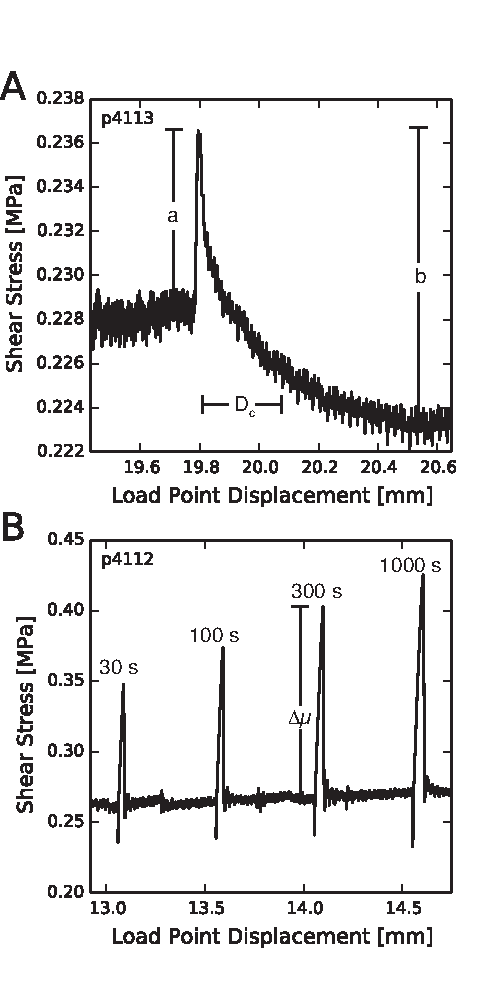
\includegraphics{chap_granular_stiffness/Fig1.pdf}
\caption{\label{fig:tests}
Experimental data showing examples of tests used to measure rate-and-state frictional parameters. (A) velocity step test in which loading velocity is changed from 150 $\mathrm{\mu}$m/s to 500 $\mathrm{\mu}$m/s. Note transient evolution of friction followed by attainment of a new steady-state. (B) results for four slide-hold-slide tests in which shearing velocity is set to zero for a period (the hold) before re-shearing, showing holds of 30, 100, 300, and 1000 seconds. Frictional healing ({}$\mu$) increases with the logarithm of hold time.}
\end{centering}
\end{figure}

\begin{figure}[t!]
\begin{centering}
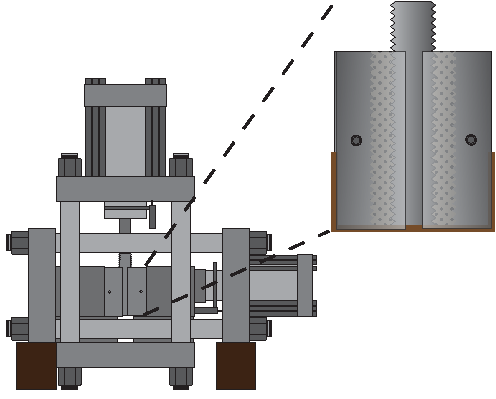
\includegraphics{chap_granular_stiffness/Fig2.pdf}
\label{fig:biax}
\caption{The biaxial press with supporting and forcing blocks in place.  Double-direct shear samples consist of three blocks: two side blocks and a center block.  Gouge layers are between the forcing blocks and confined with side-shields and a rubber membrane. (After \cite{Leeman_2014})}
\end{centering}
\end{figure}

\clearpage

\begin{figure}[t!]
\begin{centering}
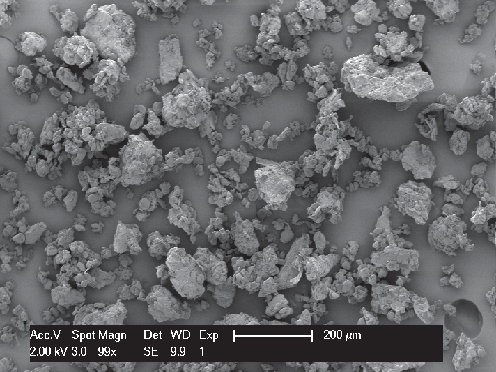
\includegraphics{chap_granular_stiffness/Fig3.pdf}
\caption{\label{fig:flour_sem}
A scanning electron micrograph of undeformed baking flour.  Grain sizes are observed to vary in the 10-200 $\mu m$ range.  The material has a platy appearance reminiscent of clay and other phyllosilicate minerals.}
\end{centering}
\end{figure}

\clearpage

\begin{figure}[t!]
\begin{centering}
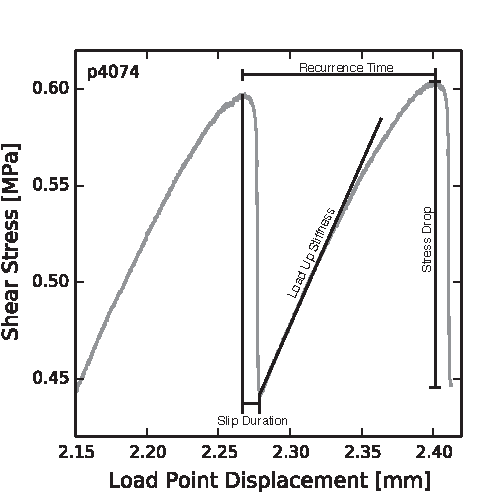
\includegraphics{chap_granular_stiffness/Fig4.pdf}
\caption{\label{fig:stickslip}
Slow-slip and stick-slip events can be characterized by their slip duration, recurrence time, stress drop, and elastic loading stiffness.  These quantities can be used to quantify the effective system stiffness and frictional properties including the rate of restrengthening (healing).    }
\end{centering}
\end{figure}



\begin{figure}
\begin{centering}
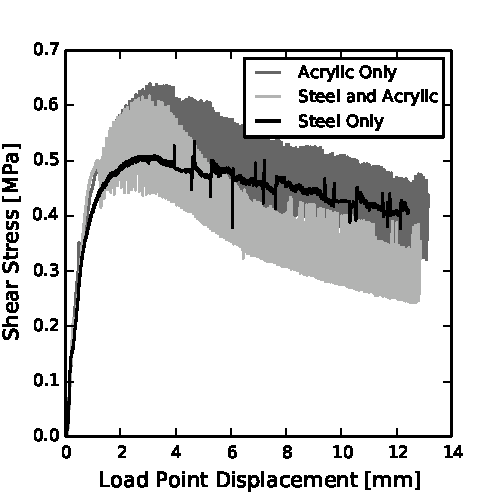
\includegraphics{chap_granular_stiffness/Fig5.pdf}
\caption{\label{fig:comp_runplots}
Data for three experiments with different forcing blocks and effective system stiffnesses.  The acrylic only and steel-acrylic experiments exhibited slow stick-slip behavior, while steel forcing blocks produced only stable sliding.}
\end{centering}
\end{figure}



\begin{figure}
\begin{centering}
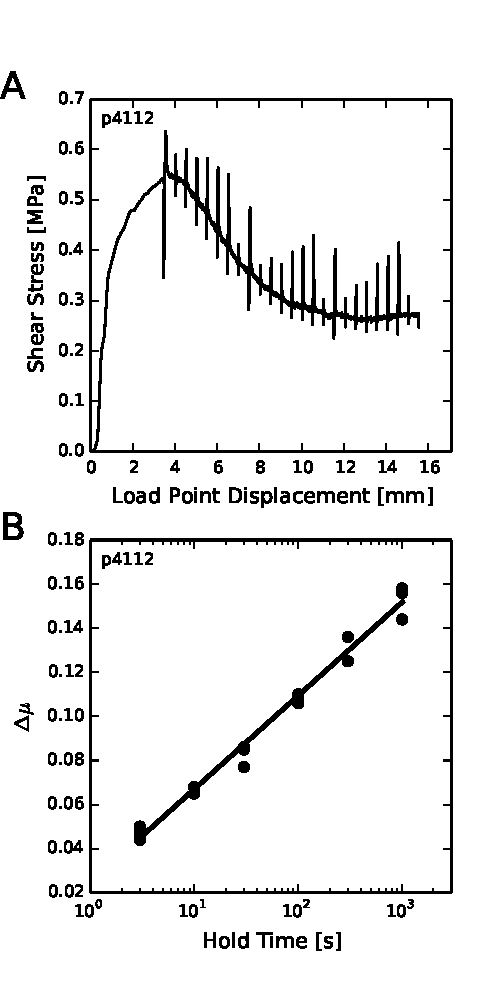
\includegraphics{chap_granular_stiffness/Fig6.pdf}
\caption{\label{fig:healing_p4112}
(A) Friction data during slide-hold-slide tests over an entire experiment with steel forcing blocks. Note initial load-up: there is a region of peak strength followed by weakening and the attainment of steady-state strength after shear of $\sim$ 10 mm.  This test included three sets of holds lasting from 3 to 1000 seconds. (B) Friction parameter $\Delta \mu$ vs. the log of hold time for the slide-hold-slide tests shown in panel A.  Healing exhibits log-linear behavior, independent of net shear displacement. }
\end{centering}
\end{figure}

\begin{figure}
\begin{centering}
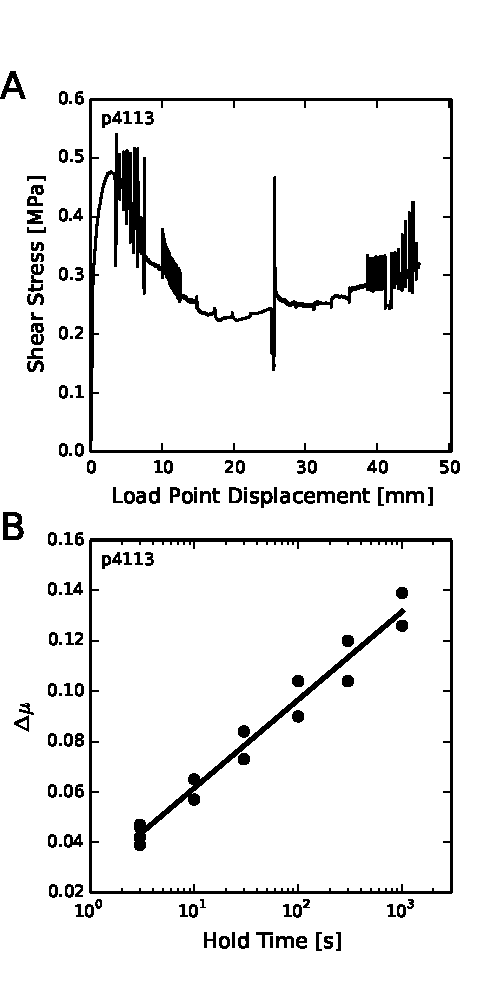
\includegraphics{chap_granular_stiffness/Fig7.pdf}
\caption{\label{fig:healing_p4113}
(A) Friction data for experiment p4113 with steel loading blocks, and (B) healing determined from slide-hold-slide tests. The sample exhibited limited stick-slip/slow-slip behavior, but only at a load point velocity of 5 $\mu m/s$.  Frictional instability appears as a wide band of noise at the scale shown, around 10 and 40 mm load point displacement. Holds ranged from 3 to 1000 seconds and velocity steps from 5 to 1500 $\mu m/s$.}
\end{centering}
\end{figure}



\begin{figure}
\begin{centering}
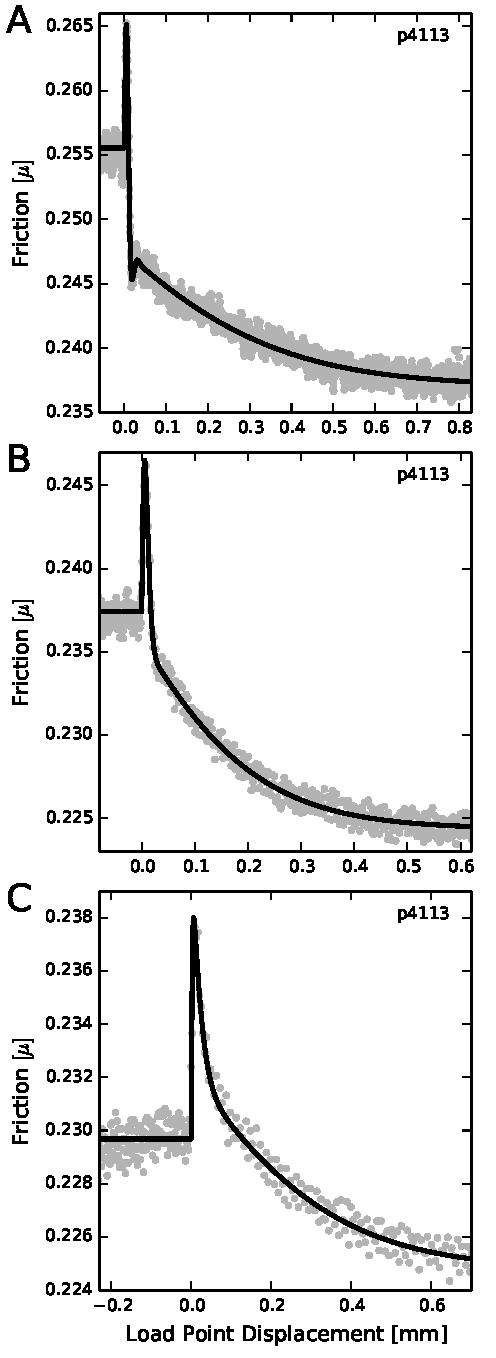
\includegraphics[scale=0.8]{chap_granular_stiffness/Fig8.pdf}
\caption{\label{fig:model_fits}
Velocity steps in an all steel forcing block configuration can only be fit by a two state variable model.  A) 15 - 50 $\mu m/s$ B) 50 - 150 $\mu m/s$ C) 150 - 500 $\mu m/s$}
\end{centering}
\end{figure}


\begin{figure}
\begin{centering}
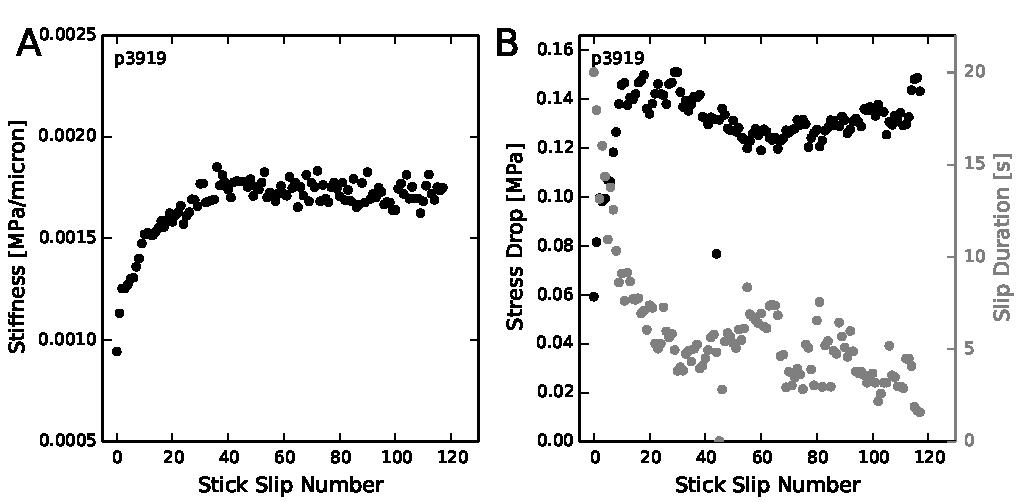
\includegraphics[scale=0.8]{chap_granular_stiffness/Fig9.pdf}
\caption{\label{fig:p3919_picks}
(A) Stiffness and (B) Stress drop and slip duration for events in experiments with all acrylic forcing blocks.  Stiffness increases on the rise to steady state by a factor of nearly two and remains remarkably constant. Stress drops rapidly increase by a factor of two over the first twenty events before reaching a steady state.  Slip duration begins at nearly twenty-five seconds, then rapidly decreases to around five seconds.}
\end{centering}
\end{figure}

\clearpage

\begin{figure}
\begin{centering}
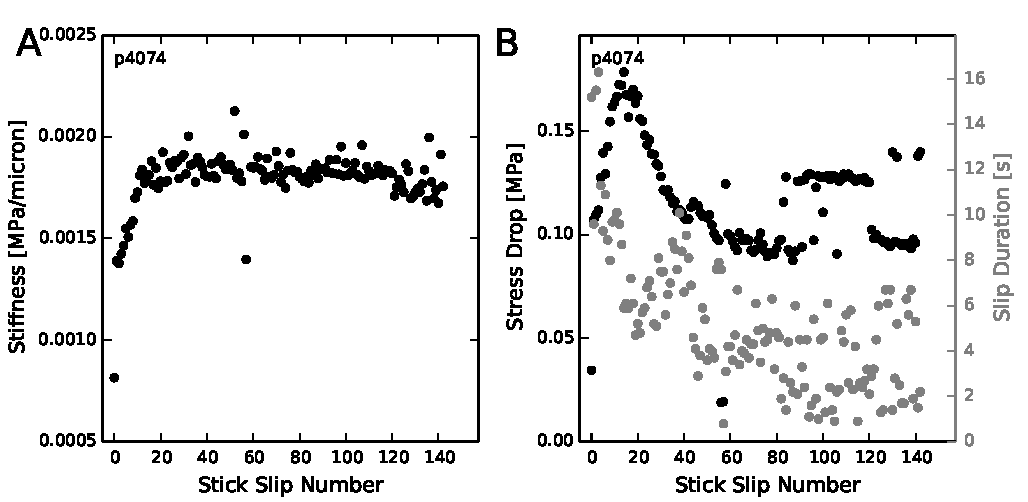
\includegraphics[scale=0.8]{chap_granular_stiffness/Fig10.pdf}
\caption{\label{fig:p4074_picks}
(A) Stiffness and (B) Stress drop and slip duration for events in the steel/acrylic forcing block system. Stiffness follows a similar trend to the all-acrylic experiment, but exhibits a smaller increase with strain. Stress drop increases rapidly, but then returns and maintains its initial level until a second family of events occurs around events 80-120.  Slip duration begins faster than for the all-acrylic blocks and stays lower with more scatter.  }
\end{centering}
\end{figure}

\begin{figure}
\begin{centering}
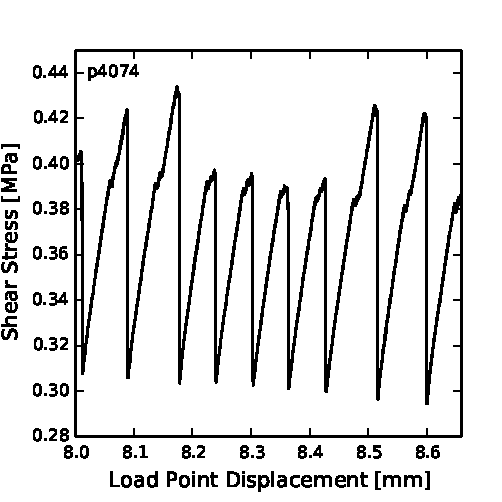
\includegraphics{chap_granular_stiffness/Fig11.pdf}
\caption{\label{fig:double_ss}
Two groups of stick-slip events are evident after sufficient shearing in the steel/acrylic system.  At the expected shear failure point there are several small failures, but the layer recovers and continues to load to a higher stress before failure.}
\end{centering}
\end{figure}


\begin{figure}
\begin{centering}
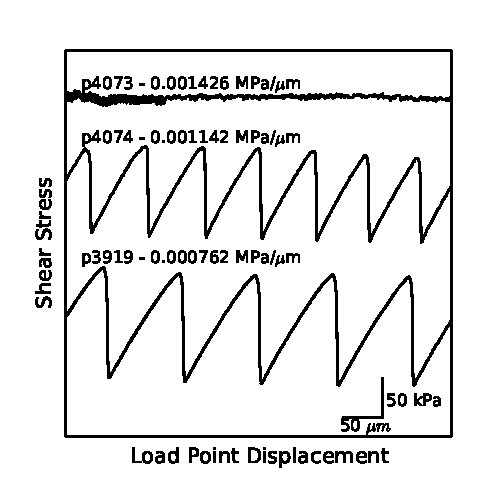
\includegraphics{chap_granular_stiffness/Fig12.pdf}
\caption{\label{fig:transition}
Response of the system with various effective stiffnesses.  The stability
boundary is crossed between the steel and steel/acrylic system.  Stiffnesses
shown are the initial load up stiffnesses of the sample.  All data are from the
same displacement range, but have been offset in shear stress for clarity. }
\end{centering}
\end{figure}

\clearpage

\begin{table}
\begin{center}
\begin{tabular}{cccccccc}
$V_0$ & $V$ & $a$ & $b_1$ & $D_{c_1}$ & $b_2$ & $D_{c_2}$ & $a-b$ \\
\hline
\hline
15&50&0.0120&0.0185&5.351&0.0088&207.912&-0.0154\\
50&150&0.0110&0.0125&7.448&0.0105&127.545&-0.0119\\
150&500&0.0077&0.0056&15.432&0.0061&199.407&-0.0041\\
\hline
\end{tabular}
\end{center}
\caption{Two state variable parameters obtained from friction data inversion with all steel forcing blocks (p4113).}
\label{rsf_params}
\end{table}

\clearpage

\begin{landscape}
\begin{table}
\begin{tabular}{cccccc}

Experiment & Blocks & Layer Thickness (mm) & Temperature (C) & Relative Humidity (\%) & Loading Stiffness (MPa/$\mu$m) \\
\hline
\hline
p3916 & Acrylic & 7 & 23.5 & 22 & 0.000630  \\
p3918 & Acrylic & 7 & 23.1 & 22 & 0.000917  \\
p3919 & Acrylic & 7 & 24.2 & 23.9 & 0.000762  \\
p3920 & Acrylic & 7 & 24.4 & 25 & 0.000871 \\
p3917 & Steel/Acrylic & 7 & 22 & 21.9 & 0.001002  \\
p4074 & Steel/Acrylic & 8 & 23.1 & 38.8 & 0.001142 \\
p4073 & Steel & 8 & 23.4 & 28.4 & 0.001426  \\
p4112 & Steel & 8 & 24.3 & 55.5 & 0.001184  \\
p4113 & Steel & 8 & 24.3 & 56.1 & 0.001070  \\
\hline
\end{tabular}
	\caption{Load up stiffnesses during run-in for different forcing block configurations.  Note that the steel/acrylic combination is much closer to the stiffness of all steel blocks than that of all acrylic blocks.}
	\label{load_stiffness}
\end{table}
\end{landscape}
